\documentclass[a4paper,11pt]{article}
\usepackage{titling}
\usepackage[left=2cm, right=2cm, top=2cm]{geometry}
\usepackage{mathtools}
\usepackage{graphicx}
\usepackage{float}
\title{\vspace{-2.0cm}EMP191 Rocket Lab 7}
\author{Warren Yuan}
\date{\today}


\begin{document}

\maketitle

\begin{abstract}
 {In this lab, students used Mathematica to make a model of and plot the trajectory of the rocket launch, based on differential equations from the force equations.}
\end{abstract}

\section{Introduction}
{\quad The goal of this lab was to be able to make an accurate model of the trajectory using Newton's laws, as well as become more well versed in Mathematica.}

\section{Measurement Procedure}
{\quad The procedure was followed through as written.}

% \section{Plots of Data}
% \begin{figure}[H]
%     \begin{center}
%     %\includegraphics[width=\linewidth/3]{}
%     \end{center}
%     \caption{Using acceleration minimum to adjust position}
%     \label{fig:Rocket Trajectory}
% \end{figure}
% \begin{figure}[H]
%     \begin{center}
%     %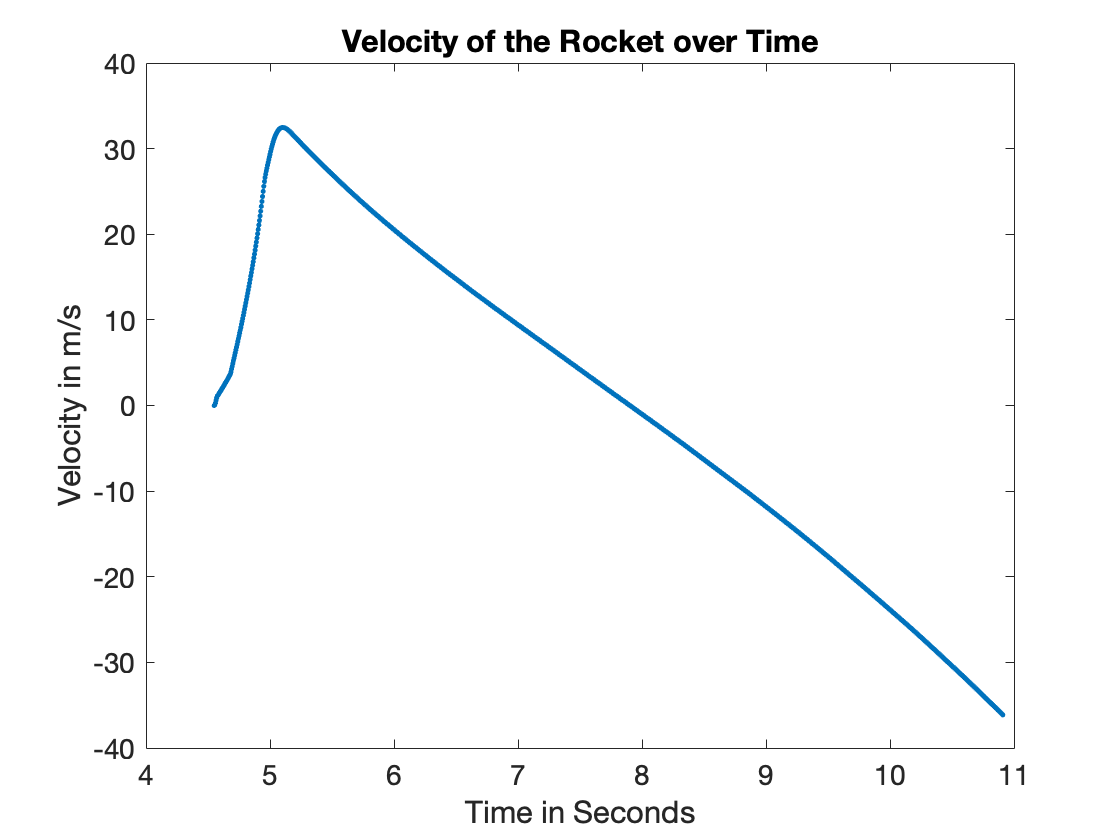
\includegraphics[width=\linewidth/3]{vel.png}
%     \end{center}
%     \caption{Graph of Velocity}
%     \label{fig:Velocity}
% \end{figure}
% \begin{figure}[H]
% \begin{center}
%     %`  1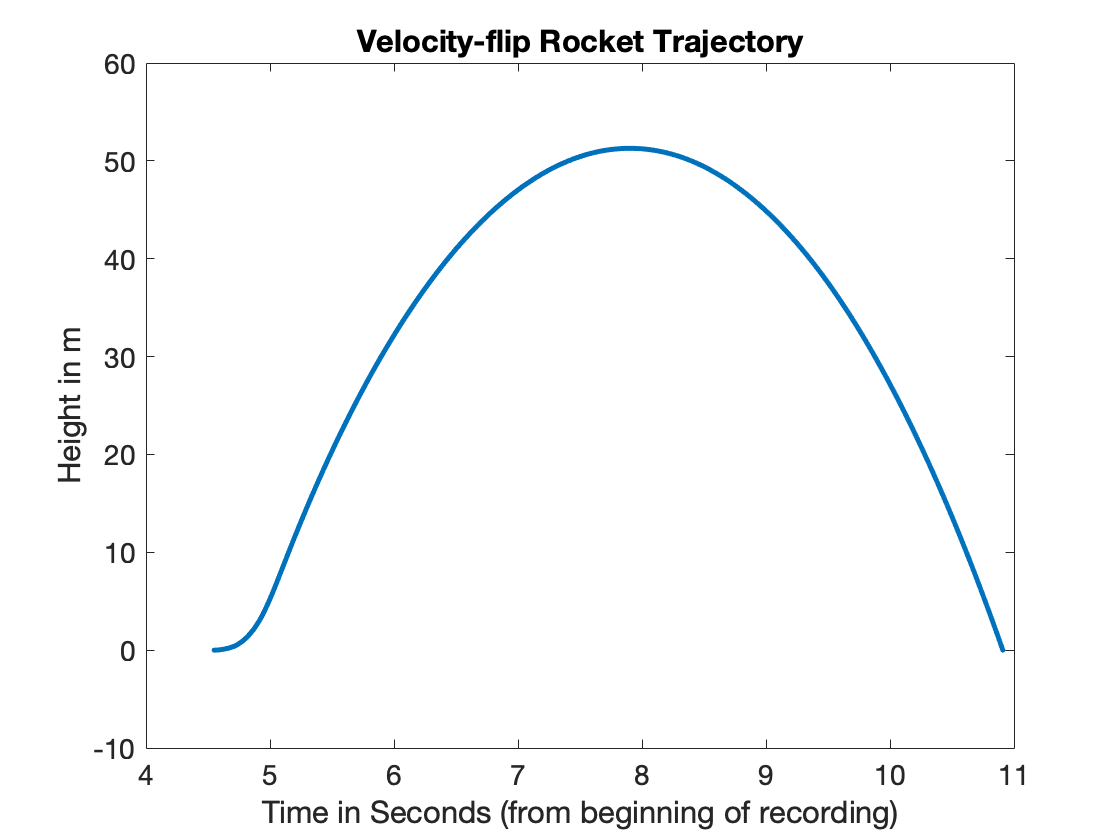
\includegraphics[width=\linewidth/3]{velrkttraj.png}
% \end{center}
%     \caption{Using Velocity sign-flip to adjust position}
%     \label{fig:Rocket Trajectory}
% \end{figure}

\section{Analysis Results}
{}
{\quad For the first part of the procedure, Oleg and I derived a series of differential equations with which we could make plots.}
{Part A: }
\begin{equation} 
    F = ma  \rightarrow \quad PA_{n} - mg = ma \rightarrow \quad a = \frac{PA_{n}}{m_{f}}-g \rightarrow \quad \frac{dv}{dt} = \frac{PA_{n}}{m_{f}}-g \rightarrow \quad 
\end{equation}
{where $m_{f}$ is the mass of the fully filled rocket.}
\begin{equation}   
    \frac{dv}{dt} = \frac{4.40*10^5*(4.75*10^{-3})^{2}*\pi}{.1889}-9.8 = 155 m/s^2
\end{equation}
\begin{equation}   
    \Delta x = v0 + at^2 \rightarrow \quad 0.22 = 0 + 155t^2 \rightarrow \quad t = 0.0377s
\end{equation}
{Part B: Using Bernoulli's Equation}
\begin{equation} 
    P_{1} + \rho gh_{1} + \frac{1}{2}\rho v_{1}^2 = P_{2} + \rho gh_{2} + \frac{1}{2}\rho v_{2}^2\rightarrow\quad  P_{1} = P_{2} + \frac{1}{2}\rho v_{2}^2\rightarrow \quad v_{2} = \sqrt{\frac{2(P_{1} - P_{2})}{\rho}}  
\end{equation}
{where $v_{2}$ is the exit velocity of the water from the rocket and $A_{n}$ is the area of the bottle nozzle.}
\begin{equation}
    v_{e} = \sqrt{\frac{2(4.40*10^5- 10^5)}{1000}} = 26.07m/s
\end{equation}
{here is the derivation of $\frac{dM}{dt}$ for 0.27 seconds until depletion.}
\begin{equation}
    \frac{dM}{dt} = Area_{nozzle} * v_{e} * 1000 = 1.84 kg/s  
\end{equation}
{Using the Rocket Equation and Newton's laws one can derive the differential equation for $\frac{dv}{dt}$.}
\begin{equation}
    \frac{dv}{dt} = \frac{2A(P_{bottle} - P_{atm})}{M_{i} - \rho v_{e} A_{n} t} - g
\end{equation}
{The drag force equation is derived below: where $A_{b}$ is the area of the bottle cross section and $m_{e}$ is the mass of the empty rocket.}
\begin{equation}
   -mg \mp kv^{2} = ma \rightarrow \quad g \pm \frac{kv^2}{m_{e}} = \frac{dv}{dt} \rightarrow \quad 
    \frac{dv}{dt} = g \pm \frac{\rho_{a} A_{b}C_{d}v_{b}^2}{2m_{e}}
\end{equation}
{Where $v_{b}$ is the velocity of the bottle and $A_{b}$,$\rho_{a}$,$C_{d}$ are the Area of the bottle, the density of air, and the C constant of drag respectively.}
\begin{figure}[H]
    %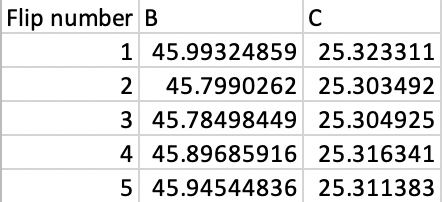
\includegraphics[width=\linewidth/4]{table.png}
\end{figure}

{}

{For Launch Tube Time : Solving for time with the equation above (and acceleration = $155m/s^2$) we get 0.0377s which is relatively close to my time of 0.0234s obtained in the previous lab. I used the times from the previous lab for the phases 2-4, getting t2 = 5.175, t3 = 7.9 seconds}

\section{Conclusion}
{Note that I was unable to obtain the graphs for to make the model. If I were, I would have been able to observe some small differences between the graph made from data from the accelerometer and that of data from the equations because of small things not taken account for (like launch angle in the simulation). }
\end{document}

